\documentclass[14pt]{beamer}
\usepackage{multimedia}

\usetheme[width=1.4cm]{PaloAlto}
\usecolortheme{default}
\useoutertheme{shadow} 

\usepackage[utf8]{inputenc}
\usepackage{booktabs,tabu}
\usepackage{adjustbox}
\usepackage{graphicx}
\usepackage{caption}
\graphicspath{{figs/}}
\DeclareGraphicsRule{.tif}{png}{.png}{`convert #1 `dirname #1`/`basename #1 .tif`.png}


%%%%%%%%%%%%%%%%%%%%
%%% BEGIN PYTHON %%%
%%%%%%%%%%%%%%%%%%%%

\usepackage{color}
\long\def\ans#1{{\color{blue}{\em #1}}}
\long\def\ansnem#1{{\color{blue}#1}}
\long\def\boldred#1{{\color{red}{\bf #1}}}

\usepackage{listings}
\usepackage{textcomp}
\renewcommand{\lstlistlistingname}{Code Listings}
\renewcommand{\lstlistingname}{Code Listing}

%%% Specific for python listings
\definecolor{gray}{gray}{0.5}
\definecolor{green}{rgb}{0,0.5,0}

\lstnewenvironment{python}[1][]{
\lstset{
language=python,
basicstyle=\tiny,
stringstyle=\color{red},
showstringspaces=false,
alsoletter={1234567890},
otherkeywords={\ , \}, \{},
keywordstyle=\color{blue},
emph={access,and,break,class,continue,def,del,elif ,else,%
except,exec,finally,for,from,global,if,import,in,i s,%
lambda,not,or,pass,print,raise,return,try,while},
emphstyle=\color{black}\bfseries,
emph={[2]True, False, None, self},
emphstyle=[2]\color{green},
emph={[3]from, import, as},
emphstyle=[3]\color{blue},
upquote=true,
morecomment=[s]{"""}{"""},
commentstyle=\color{gray}\slshape,
emph={[4]1, 2, 3, 4, 5, 6, 7, 8, 9, 0},
emphstyle=[4]\color{blue},
literate=*{:}{{\textcolor{blue}:}}{1}%
{=}{{\textcolor{blue}=}}{1}%
{-}{{\textcolor{blue}-}}{1}%
{+}{{\textcolor{blue}+}}{1}%
{*}{{\textcolor{blue}*}}{1}%
{!}{{\textcolor{blue}!}}{1}%
{(}{{\textcolor{blue}(}}{1}%
{)}{{\textcolor{blue})}}{1}%
{[}{{\textcolor{blue}[}}{1}%
{]}{{\textcolor{blue}]}}{1}%
{<}{{\textcolor{blue}<}}{1}%
{>}{{\textcolor{blue}>}}{1},%
%framexleftmargin=1mm, framextopmargin=1mm, frame=shadowbox, rulesepcolor=\color{blue},#1
framexleftmargin=1mm, framextopmargin=1mm, frame=single,#1
}}{}

%%%%%%%%%%%%%%%%%%
%%% END PYTHON %%%
%%%%%%%%%%%%%%%%%%


% remove navigation symbols
\setbeamertemplate{navigation symbols}{}
\setbeamerfont{page number in head/foot}{size=\fontsize{12}{12}}
\setbeamertemplate{footline}[frame number]

% make image sized to frame
\newcommand {\framedgraphic}[2] { % args = {frametitle}{image.ext}
    \begin{frame}{#1}
        \begin{center}
            \includegraphics[width=\textwidth,height=0.8\textheight,keepaspectratio]{#2}
        \end{center}
    \end{frame}
}

% This block will remove authornames and talk title from sidebar
\makeatletter
  \setbeamertemplate{sidebar \beamer@sidebarside}%{sidebar theme}
  {
    \beamer@tempdim=\beamer@sidebarwidth%
    \advance\beamer@tempdim by -6pt%
    \insertverticalnavigation{\beamer@sidebarwidth}%
    \vfill
    \ifx\beamer@sidebarside\beamer@lefttext%
    \else%
      \usebeamercolor{normal text}%
      \llap{\usebeamertemplate***{navigation symbols}\hskip0.1cm}%
      \vskip2pt%
    \fi%
}%
\makeatother




\begin{document}

\title{A TensorFlow Tutorial}  
\subtitle{Email Classification with Logistic Regression}
\author{Josh Meyer \inst{1} \and Michael Capizzi \inst{2}}
\institute{ \inst{1} University of Arizona \and \inst{2} PitchVantage}
\date{} 

\frame{\titlepage} 

\frame{\frametitle{Table of contents}\tableofcontents} 


\section{What's Going to Happen}

\frame{
Tonight we will...
\begin{itemize}
\item describe the basic TensorFlow structures
\item build a working example of text classification
\item point out places where \textit{other} TensorFlow "built-ins" apply {\footnotesize(optimizers, cost functions, etc)}
\item "hand-wave" liberally \\
{\footnotesize(when we don't want to get into it or don't know the answer)}
\end{itemize}
Tonight we will \textbf{not}...
\begin{itemize}
\item discuss details of NLP feature selection
\item discuss details of Machine Learning \\
{\footnotesize(linear algebra, backpropogation, etc.)}
\end{itemize}
}

\section{TensorFlow Structures}

\frame{\frametitle{}
  \centering
    \begingroup
    \fontsize{20pt}{20pt}\selectfont
    TensorFlow Structures
  \endgroup
  \begin{flushleft}
  tensor = \textit{n}-dimensional matrix
  \end{flushleft}
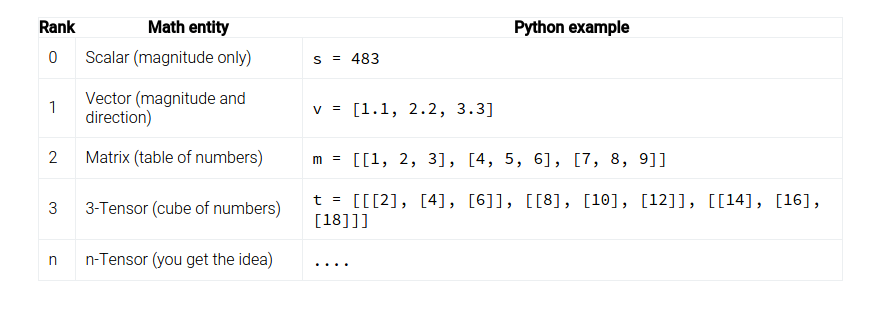
\includegraphics[width=\textwidth,height=0.9\textheight,keepaspectratio]{tensors.png}}

\begin{frame}[fragile]
\frametitle{TensorFlow Structures}
\begin{itemize}
\item{\textbf{constants}}: {\small \textit{never} changes its value(s)} \\
\begin{python}
c = tf.constant(2.0, name="constantC") #can be int, float, or tensor
\end{python}
\item{\textbf{placeholders}}: {\small shell into which tensors can be iteratively inserted} \\
\begin{python}
X = tf.placeholder(tf.float32, [None, 200], name="input")
\end{python}
\item{\textbf{variables}}: {\small value(s) can be updated}
\begin{python}
weights = tf.Variable(tf.random_normal([1, 200], name="weights"))
\end{python}
\item{\textbf{operations}}: {\small computations that will act on tensors}
\begin{python}
apply_weights_OP = tf.matmul(X, weights, name="apply_weights")
add_bias_OP = tf.add(apply_weights_OP, bias, name="add_bias")
activation_OP = tf.nn.sigmoid(add_bias_OP, name="activation")\end{python}
\end{itemize}
\end{frame}

\section{The Flow of TensorFlow}

\frame{\frametitle{}
  \centering
    \begingroup
    \fontsize{20pt}{20pt}\selectfont
    Let's get to the script!\\
  \endgroup
}

\begin{frame}[fragile]
  \frametitle{Preamble}
  \begin{python}
################
### PREAMBLE ###
################

from __future__ import division
import tensorflow as tf
import numpy as np
import tarfile
import os
import matplotlib.pyplot as plt
import time
  \end{python}
\end{frame}


\begin{frame}[fragile]
  \frametitle{Import the Email Data}
  \begin{python}
###################
### IMPORT DATA ###
###################

def csv_to_numpy_array(filePath, delimiter):
    return np.genfromtxt(filePath, delimiter=delimiter, dtype=None)

def import_data():
    if "data" not in os.listdir(os.getcwd()):
        # Untar directory of data if we haven't already
        tarObject = tarfile.open("data.tar.gz")
        tarObject.extractall()
        tarObject.close()
        print("Extracted tar to current directory")
    else:
        # we've already extracted the files
        pass

    print("loading training data")
    trainX = csv_to_numpy_array("data/trainX.csv", delimiter="\t")
    trainY = csv_to_numpy_array("data/trainY.csv", delimiter="\t")
    print("loading test data")
    testX = csv_to_numpy_array("data/testX.csv", delimiter="\t")
    testY = csv_to_numpy_array("data/testY.csv", delimiter="\t")
    return trainX,trainY,testX,testY

trainX,trainY,testX,testY = import_data()
  \end{python}
\end{frame}



\begin{frame}[fragile]
  \frametitle{Some Global Parameters}
  \begin{python}
#########################
### GLOBAL PARAMETERS ###
#########################

# DATA SET PARAMETERS
# Get our dimensions for our different variables and placeholders:
# numFeatures = the number of words extracted from each email
numFeatures = trainX.shape[1]
# numLabels = number of classes we are predicting (here just 2: Ham or Spam)
numLabels = trainY.shape[1]

# TRAINING SESSION PARAMETERS
# number of times we iterate through training data
# tensorboard shows that accuracy plateaus at ~25k epochs
numEpochs = 27000
# a smarter learning rate for gradientOptimizer
learningRate = tf.train.exponential_decay(learning_rate=0.0008,
                                          global_step= 1,
                                          decay_steps=trainX.shape[0],
                                          decay_rate= 0.95,
                                          staircase=True)
  \end{python}
\end{frame}

\frame{\frametitle{}
  \centering
    \begingroup
    \fontsize{20pt}{20pt}\selectfont
    The Computational Graph\\
  \endgroup
}


\framedgraphic{The Full Computational Graph}{full-graph.png}

\framedgraphic{Define Feature and Label Placeholders}{define-X-Y-matrices.png}

\begin{frame}[fragile]
  \frametitle{Define Feature and Label Placeholders}
  \begin{python}
####################
### PLACEHOLDERS ###
####################

# X = X-matrix / feature-matrix / data-matrix... It's a tensor to hold our
# email data. 'None' here means that we can hold any number of emails
X = tf.placeholder(tf.float32, [None, numFeatures])

# yGold = Y-matrix / label-matrix / labels... This will be our correct answers
# matrix. Every row has either [1,0] for SPAM or [0,1] for HAM. 'None' here 
# means that we can hold any number of emails
yGold = tf.placeholder(tf.float32, [None, numLabels])
  \end{python}
\end{frame}


\framedgraphic{Initialize Weights \& Bias Terms Op}{1-initialization.png}

\begin{frame}[fragile]
  \frametitle{Initialize Weights \& Bias Terms Op}
  \begin{python}
#################
### VARIABLES ###
#################

# all values are randomly assigned:
# sqrt(6 / (numInputNodes + numOutputNodes + 1))

weights = tf.Variable(tf.random_normal([numFeatures,numLabels],
          mean=0,
          stddev=(np.sqrt(6/numFeatures+numLabels+1)),
          name="weights"))

bias = tf.Variable(tf.random_normal([1,numLabels],
       mean=0,
       stddev=(np.sqrt(6/numFeatures+numLabels+1)),
       name="bias"))


# INITIALIZE our weights and biases
init_OP = tf.initialize_all_variables()
  \end{python}
\end{frame}


\framedgraphic{Apply Weights to Features Op}{2-apply-weights.png}

\begin{frame}[fragile]
  \frametitle{Apply Weights to Features Op}
  \begin{python}
apply_weights_OP = tf.matmul(X, weights, name="apply_weights")
  \end{python}
\end{frame}


\framedgraphic{Add Bias to Weighted Features Op}{3-add-bias.png}

\begin{frame}[fragile]
  \frametitle{Add Bias to Weighted Features Op}
  \begin{python}
add_bias_OP = tf.add(apply_weights_OP, bias, name="add_bias") 
  \end{python}
\end{frame}


\framedgraphic{Activation Op}{4-apply-sigmoid.png}

\begin{frame}[fragile]
  \frametitle{Activation Op}
  \begin{python}
activation_OP = tf.nn.sigmoid(add_bias_OP, name="activation")
  \end{python}
\end{frame}


\framedgraphic{Evaluation Op: Mean Squared Error}{5-loss-function.png}

\begin{frame}[fragile]
  \frametitle{Evaluation Op: Mean Squared Error}
  \begin{python}
#####################
### EVALUATION OP ###
#####################

# COST FUNCTION i.e. MEAN SQUARED ERROR
cost_OP = tf.nn.l2_loss(activation_OP-yGold, name="squared_error_cost")  \end{python}
\end{frame}

\framedgraphic{Optimization Op: Gradient Descent}{6-optimization.png}

\begin{frame}[fragile]
  \frametitle{Optimization Op: Gradient Descent}
  \begin{python}
#######################
### OPTIMIZATION OP ###
#######################

# OPTIMIZATION ALGORITHM i.e. GRADIENT DESCENT
training_OP = tf.train.GradientDescentOptimizer(learningRate).minimize(cost_OP)
  \end{python}
\end{frame}



\begin{frame}[fragile]
  \frametitle{Run the Graph}
  \begin{python}
#####################
### RUN THE GRAPH ###
#####################

# Create a tensorflow session
sess = tf.Session()
# Initialize all tensorflow variables
sess.run(init_OP)

## Ops for vizualization
# argmax(activation_OP, 1) gives the label our model thought was most likely
# argmax(yGold, 1) is the correct label
correct_predictions_OP=tf.equal(tf.argmax(activation_OP,1),tf.argmax(yGold,1))
# False is 0 and True is 1, what was our average?
accuracy_OP = tf.reduce_mean(tf.cast(correct_predictions_OP, "float"))
# Summary op for regression output
activation_summary_OP = tf.histogram_summary("output", activation_OP)
# Summary op for accuracy
accuracy_summary_OP = tf.scalar_summary("accuracy", accuracy_OP)
# Summary op for cost
cost_summary_OP = tf.scalar_summary("cost", cost_OP)
# Summary ops to check how variables (W, b) are updating after each iteration
weightSummary = tf.histogram_summary("weights", weights.eval(session=sess))
biasSummary = tf.histogram_summary("biases", bias.eval(session=sess))
# Merge all summaries
all_summary_OPS = tf.merge_all_summaries()
# Summary writer
writer = tf.train.SummaryWriter("summary_logs", sess.graph_def)
  \end{python}
\end{frame}

\begin{frame}[fragile]
  \frametitle{Still 'Running the Graph'}
  \begin{python}
# Initialize reporting variables
cost = 0
diff = 1
# Training epochs
for i in range(numEpochs):
    if i > 1 and diff < .0001:
        print("change in cost %g; convergence."%diff)
        break
    else:
        # Run training step
        step = sess.run(training_OP, feed_dict={X: trainX, yGold: trainY})
        # Report occasional stats
        if i % 10 == 0:
            # Add epoch to epoch_values
            epoch_values.append(i)
            # Generate accuracy stats on test data
            summary_results, train_accuracy, newCost = sess.run(
                [all_summary_OPS, accuracy_OP, cost_OP], 
                feed_dict={X: trainX, yGold: trainY}
            )
            # Add accuracy to live graphing variable
            accuracy_values.append(train_accuracy)
            # Add cost to live graphing variable
            cost_values.append(newCost)
            # Write summary stats to writer
            writer.add_summary(summary_results, i)
            # Re-assign values for variables
            diff = abs(newCost - cost)
            cost = newCost
  \end{python}
\end{frame}

\begin{frame}[fragile]
  \frametitle{Still 'Still Running the Graph'}
  \begin{python}
            #generate print statements
            print("step %d, training accuracy %g"%(i, train_accuracy))
            print("step %d, cost %g"%(i, newCost))
            print("step %d, change in cost %g"%(i, diff))

            # Plot progress to our two subplots
            accuracyLine, = ax1.plot(epoch_values, accuracy_values)
            costLine, = ax2.plot(epoch_values, cost_values)
            fig.canvas.draw()
            time.sleep(1)


# How well do we perform on held-out test data?
print("final accuracy on test set: %s" %str(sess.run(accuracy_OP, 
                                                 feed_dict={X: testX, 
                                                        yGold: testY})))
  \end{python}
\end{frame}

\begin{frame}[fragile]
  \frametitle{Reuse, Recycle}
  \begin{python}
##############################
### SAVE TRAINED VARIABLES ###
##############################

# Create Saver
saver = tf.train.Saver()
# Save variables to .ckpt file
# saver.save(sess, "trained_variables.ckpt")

# Close tensorflow session
sess.close()
  \end{python}
\end{frame}

\framedgraphic{}{thats-all-folks.jpg}


\end{document}
